
\documentclass[twoside]{article}
% \documentclass[twoside,twocolumn]{article}

\usepackage{blindtext} % Package to generate dummy text throughout this template 

\usepackage[sc]{mathpazo} % Use the Palatino font
\usepackage[T1]{fontenc} % Use 8-bit encoding that has 256 glyphs
\linespread{1.05} % Line spacing - Palatino needs more space between lines
\usepackage{microtype} % Slightly tweak font spacing for aesthetics

\usepackage[english]{babel} % Language hyphenation and typographical rules

\usepackage[hmarginratio=1:1,top=32mm,columnsep=20pt]{geometry} % Document margins
\usepackage[hang, small,labelfont=bf,up,textfont=it,up]{caption} % Custom captions under/above floats in tables or figures
\usepackage{booktabs} % Horizontal rules in tables

\usepackage{lettrine} % The lettrine is the first enlarged letter at the beginning of the text

\usepackage{enumitem} % Customized lists
\setlist[itemize]{noitemsep} % Make itemize lists more compact

\usepackage{abstract} % Allows abstract customization
\renewcommand{\abstractnamefont}{\normalfont\bfseries} % Set the "Abstract" text to bold
\renewcommand{\abstracttextfont}{\normalfont\small\itshape} % Set the abstract itself to small italic text

\usepackage{titlesec} % Allows customization of titles
\renewcommand\thesection{\Roman{section}} % Roman numerals for the sections
\renewcommand\thesubsection{\roman{subsection}} % roman numerals for subsections
\titleformat{\section}[block]{\large\scshape\centering}{\thesection.}{1em}{} % Change the look of the section titles
\titleformat{\subsection}[block]{\large}{\thesubsection.}{1em}{} % Change the look of the section titles

\usepackage{fancyhdr} % Headers and footers
\pagestyle{fancy} % All pages have headers and footers
\fancyhead{} % Blank out the default header
\fancyfoot{} % Blank out the default footer
\fancyhead[C]{CSE539 $\bullet$ Applied Cryptography $\bullet$ Project Report $\bullet$ AES Implementation $\bullet$ Fall 2017} % Custom header text
\fancyfoot[RO,LE]{\thepage} % Custom footer text

\usepackage{titling} % Customizing the title section

\usepackage{hyperref} % For hyperlinks in the PDF

\usepackage{graphicx}
\graphicspath{ {images/} }

%----------------------------------------------------------------------------------------
%	TITLE SECTION
%----------------------------------------------------------------------------------------

\setlength{\droptitle}{-4\baselineskip} % Move the title up

\pretitle{\begin{center}\Huge\bfseries} % Article title formatting
\posttitle{\end{center}} % Article title closing formatting
\title{%
  CSE 539 Project Report \\
  \large "Implementation of Advanced Encryption Standard (AES)"} % Article title
  
\author{%
\textsc{Anthony Pipia} \\[1ex] % Author 2 name
\normalsize Arizona State University \\ % Author 2 institution
\normalsize \href{mailto:Anthony.Pipia@asu.edu}{Anthony.Pipia@asu.edu} % Author 2 email address
\and
\textsc{Suchita Vichare} \\[1ex] % Author 2 name
\normalsize Arizona State University \\ % Author 2 institution
\normalsize \href{mailto:ssvichar@asu.edu}{ssvichar@asu.edu} % Author 2 email address
\and
\textsc{Tariq M Nasim} \\[1ex] % Author 1 name
\normalsize Arizona State University \\ % Author 1 institution
\normalsize \href{mailto:tnasim@asu.edu}{tnasim@asu.edu} % Author 1 email address
}
\date{\today} % Leave empty to omit a date
\renewcommand{\maketitlehookd}{%

}

%----------------------------------------------------------------------------------------

\begin{document}

% Print the title
\maketitle

%----------------------------------------------------------------------------------------
%	ARTICLE CONTENTS
%----------------------------------------------------------------------------------------

\section{Introduction}

In this project we have implemented the Advanced Encryption Standard (AES) for 128 bit key size and 128 bit block size. \textbf{\textit{\underline{MORE DESCRIPTION NEEDED ... }}}

%------------------------------------------------

\section{Implementation Description}

C++ programming language has been used for the implementation. The implementation has been done from scratch, i.e. without taking help from any third party library related to cryptography or AES. The important steps of implementation are:
\begin{itemize}
	\item The C++ project structure:
	\item 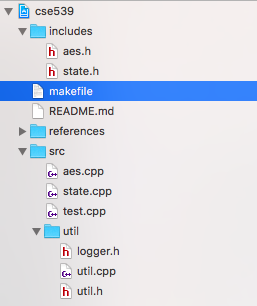
\includegraphics{project_structure_xcode}
	\item since C++ does not have data type named 'byte', we have used 'unsigned char' in all places where we needed to use byte (8-bit data).
	\item A class state has been defined that contains the operations required to be performed on a state. The state has been defined as a two dimensional array of bytes (i.e. unsigned char)
	\item class AES contains the necessary functions specific to the AES operations. The AES class actually calls the methods of 'state' class to perform operations that only involves working with the state array, i.e. the operations 'Inv/SubBytes()', 'Inv/ShiftRows()', 'Inv/MixColumns()' and 'AddRoundKey()' etc are performed through the 'state' class. The AES class does not contain the actual implementation of those methods. The methods that the AES class actually implements are the following:
	\begin{itemize}
		\item KeyExpansion: It takes as input the original key of size 128 bit and expands the key into a key schedule of size $(Nb \times (Nr+1) = 4\times (10+1)=44$ words i.e. $44\times 4 = 176$ bytes.
		\item Cipher: using the state operations, it performs the actual cipher operation.
		\item InvCipher: it performs the inverses cipher operations using the inverse state operations (InvSubBytes(), InvShiftRows(), InvMixColums) and the AddRoundKey() operation.
	\end{itemize}
	\item class util contains some important utility operations and structure definition:
	\begin{itemize}
		\item method charToHex
		\item method hexToChar
		\item structure 'word': since there is no 'word' data type in C++, we have defined a word structure. A word is a 4 byte data. We have defined it using an array of 4 'unsigned char's. The word structure also contains some important operations that needs to be performed on words:
		\begin{itemize}
			\item subWord(): ...
			\item rotWord(): ...
			\item XOR ($\oplus$) operator has been defined on full words by operator overloading.
			\item equal (==) and not-equal (!=) operators have been defined on full words by operator overloading.
		\end{itemize}
	\end{itemize}
\end{itemize}

%------------------------------------------------

\section{Crypto Learning}
We have learnt the following important aspects of cryptography through the implementation of AES in this project:
\begin{itemize}
\item \textbf{Encryption/Decryption:} The purpose of encryption is to transform an input data into a different form so that it becomes difficult to retrieve the original data withouth having the actual key that has been used for encryption. The strength of an encryption scheme is measured by the level of difficulty it introduces by the encryption. AES is an encryption scheme that is being widely used now-a-days throughout the world. In this implementation we have studied about the design of this encryption algorithm and also learnt how to implement it appropriately.
\item \textbf{Block Cyphers:} Plaintexts are divided into multiple blocks. Individual blocks are chosen and some steps of operations are applied on the blocks. A key (or part of expanded key) is used to alter the data in each block.
\item \textbf{Key Expansion:} We have learnt how to expand a small key to construct a larger one. ...
\item \textbf{Block Chaining:} Though we have not implemented it, we have studied on the ways how to encrypt/decrypt messages of length greater than the block length for the encryption scheme. ...
\end{itemize}

%------------------------------------------------

\section{Secure Coding}
Secure Coding

\section{Summary}
Summary

%----------------------------------------------------------------------------------------
%	REFERENCE LIST
%----------------------------------------------------------------------------------------

\begin{thebibliography}{99} 

\bibitem[1]{auto}
Joan Daemen and Vincent Rijmen, AES submission document on Rijndael, June 1998

\bibitem[2]{auto}
Joan Daemen and Vincent Rijmen, AES submission document on Rijndael, Version 2, September 1999
\newblock \url{http://csrc.nist.gov/CryptoToolkit/aes/rijndael/Rijndael.pdf}

\bibitem[3]{auto}
FIPS PUB 197, Advanced Encryption Standard (AES), National Institute of Standards and Technology, U.S. Department of Commerce, November 2001.
\newblock \url{http://csrc.nist.gov/publications/fips/fips197/fips-197.pdf}

\bibitem[4]{auto}
Joan Daemen and Vincent Rijmen, The Design of Rijndael AES - The Advanced Encryption Standard November 26, 2001.
\newblock \url{https://pdfs.semanticscholar.org/d440/7ce703cc42e2578a09f9352e686fc47775da.pdf}

\bibitem[5]{auto}
Alex Biryukov and Adi Shamir, Structural Cryptanalysis of SASAS, Advances in Cryptology, Proc. Eurocrypt'01, LNCS 2045, B. Pfitzmann, Ed., SpringerVerlag, 2001, pp. 394-405

\bibitem[6]{auto}
J. Daemen, L. Knudsen, V. Rijmen, The Block Cipher Square, proceedings of FSE?97, LNCS 1267, pp.147-165, Springer-Verlag, 1997.

\bibitem[7]{auto}
Carlos Cid, Sean Murphy, and Matthew Robshaw, Algebraic Aspects of the Advanced Encryption Standard, Springer, 2006

\bibitem[8]{auto}
Nicolas Courtois and Josef Pieprzyk , Cryptanalysis of Block Ciphers with Overdefined Systems of Equations, Cryptology ePrint Archive 2002/044, 2002

\bibitem[9]{auto}
H. Demirci and A. A. Sel'cuk. A Meet-in-the-Middle Attack on 8-Round AES. In Nyberg [23], pages 116-126.

\bibitem[10]{auto}
H. Demirci, I. Taskin, M. C'oban, and A. Baysal. Improved Meet-in-the-Middle Attacks on AES. In B. K. Roy and N. Sendrier, editors, INDOCRYPT, volume 5922 of Lecture Notes in Computer Science, pages 144-156. Springer, 2009.

\bibitem[11]{auto}
Li Rongjia and Jin Chenhui. Meet-in-the-middle attacks on 10-round AES-256. Designs, Codes and Cryptography, pages 113, 2015.

\bibitem[12]{auto}
O. Dunkelman, N. Keller, and A. Shamir. Improved Single-Key Attacks on 8- Round AES-192 and AES-256. In Masayuki Abe, editor, ASIACRYPT, volume 6477 of Lecture Notes in Computer Science, pages 158-176. Springer, 2010.

\bibitem[13]{auto}
A. Biryukov, D. Khovratovich, Related-key cryptanalysis of the full AES-192 and AES-256. in M. Matsui (Ed.): Asiacrypt 2009, LNCS 5912, PP.1-18, 2009.

\bibitem[14]{auto}
B. Bahrak, M. Reza Aref. Impossible Differential Attack on Seven-RoundAES-128, IET Information Security journal, Vol. 2, Number 2, pp. 28-32, IET, 2008. 

\bibitem[15]{auto}
Z. Yuan, New Impossible Differential Attacks on AES, Beijing Electronic Science and Technology Institute, Beijing, China.
\newblock \url{http://eprint.iacr.org/2010/093.pdf}

\bibitem[16]{auto}
Andrey Bogdanov, Dmitry Khovratovich, and Christian Rechberger. Biclique cryptanalysis of the full AES. Cryptology ePrint Archive, Report 2011/449, 2011.
\newblock \url{http://eprint.iacr.org/2011/449, to appear in ASIACRYPT 2011}

\bibitem[17]{auto}
A. Bogdanov, Improved Side-Channel Collision Attacks on AES, in the proceedings of SAC 2007, LNCS, vol 4876, pp 84-95, Ottawa, Canada, August 2007.

\bibitem[18]{auto}
K. Schramm, G. Leander, P. Felke, C. Paar, A Collision-Attack on AES: Combining Side Channel and Differential Attack, in the proceedings of CHES 2004, LNCS, vol 3156, pp 163-175, Cambridge, MA, USA, August 2004

\bibitem[19]{auto}
Biryukov, A., Khovratovich, D., Nikoli?c, I.: Distinguisher and related-key attack on the full AES-256. In: Halevi, S. (ed.) CRYPTO 2009. LNCS, vol. 5677, pp. 231?249. Springer, Heidelberg (2009)

\bibitem[20]{auto}
Biham, E.: New types of cryptanalytic attacks using related keys. J. Cryptology 7(4), 229-246 (1994)

\bibitem[21]{auto}
Dinur, I., Shamir, A.: Side Channel Cube Attacks on Block Ciphers. Cryptology ePrint Archive, Report 2009/127 (2009),
\newblock \url{http://eprint.iacr.org/2009/127}

\bibitem[22]{auto}
D. Bernstein. Cache-timing attacks on AES.
\newblock \url{http://cr.yp.to/papers.html\#cachetiming, 2005}

\bibitem[23]{auto}
SEI CERT C++ Coding Standard, Software Engineering Institution, Carnegie Mellon University.
\newblock \url{https://www.securecoding.cert.org/confluence/pages/viewpage.action?pageId=637}

\end{thebibliography}

\section{More Reference}
Report on the Development of the Advanced Encryption Standard (AES)\\
https://csrc.nist.gov/publications/detail/journal-article/2001/report-on-the-development-of-the-aes\\

Status Report on the First Round of the Development of the Advanced Encryption Standard (AES)
https://csrc.nist.gov/publications/detail/journal-article/1999/first-round-status-report-on-aes-development

%----------------------------------------------------------------------------------------

\end{document}


